% ******************************************************** %
%              TEMPLATE DE INFORME ORGA2 v0.1              %
% ******************************************************** %
% ******************************************************** %
%                                                          %
% ALGUNOS PAQUETES REQUERIDOS (EN UBUNTU):                 %
% ========================================
%                                                          %
% texlive-latex-base                                       %
% texlive-latex-recommended                                %
% texlive-fonts-recommended                                %
% texlive-latex-extra?                                     %
% texlive-lang-spanish (en ubuntu 13.10)                   %
% ******************************************************** %


\documentclass[a4paper]{article}
\usepackage[spanish]{babel}
\usepackage[utf8]{inputenc}
\usepackage{charter}   % tipografia
\usepackage{graphicx}
\usepackage[table,xcdraw]{xcolor}
%\usepackage{makeidx}
\usepackage{paralist} %itemize inline

\usepackage{float}
\usepackage{amsmath, amsthm, amssymb}
\usepackage{amsfonts}
%\usepackage{sectsty}
%\usepackage{charter}
%\usepackage{wrapfig}
\usepackage{listingsutf8}

% \setcounter{secnumdepth}{2}
\usepackage{underscore}
\usepackage{caratula}
\usepackage{url}
%\usepackage[superscript,biblabel]{cite}
%\usepackage{dibujitos}

\usepackage{ textcomp }

\usepackage{amssymb}
\usepackage{hyperref}


\graphicspath{ {img/} {../graph/} }

% ********************************************************* %
% ~~~~~~~~              Code snippets             ~~~~~~~~~ %
% ********************************************************* %

\usepackage{color} % para snipets de codigo coloreados
\usepackage{fancybox}  % para el sbox de los snipets de codigo

\definecolor{litegrey}{gray}{0.94}

\newenvironment{codesnippet}{%
	\begin{Sbox}\begin{minipage}{\textwidth}\sffamily\small}%
	{\end{minipage}\end{Sbox}%
		\begin{center}%
		\vspace{-0.4cm}\colorbox{litegrey}{\TheSbox}\end{center}\vspace{0.3cm}}

\definecolor{mygreen}{rgb}{0,0.6,0}
\definecolor{mygray}{rgb}{0.5,0.5,0.5}
\definecolor{mymauve}{rgb}{0.58,0,0.82}

\lstset{ %
  backgroundcolor=\color{litegrey},
  basicstyle=\footnotesize,
  breakatwhitespace=true,
  breaklines=true,
  captionpos=b,                    % sets the caption-position to bottom
  mathescape=true,
  keepspaces=true,
  language=Python,
  showspaces=false,
  tabsize=2,                       % sets default tabsize to 2 spaces
  inputencoding=utf8/latin1
}

\newcommand{\cuidado}{{\large $\Delta$!!!} \hspace*{1em}}

\newcommand*{\QEDA}{\hfill\ensuremath{\blacksquare}}%
\newcommand*{\QEDB}{\hfill\ensuremath{\square}}%

% ********************************************************* %
% ~~~~~~~~         Formato de las páginas         ~~~~~~~~~ %
% ********************************************************* %

\usepackage{fancyhdr}
\pagestyle{fancy}

\renewcommand{\sectionmark}[1]{\markright{\thesection\ - #1}}

\fancyhf{}

\fancyhead[LO]{Sección \rightmark} % \thesection\
\fancyfoot[LO]{\small{Agustín Borgna, Alan Corleto, Franco Lancioni, Luis Badell}}
\fancyfoot[RO]{\thepage}
\renewcommand{\headrulewidth}{0.5pt}
\renewcommand{\footrulewidth}{0.5pt}
\setlength{\hoffset}{-0.8in}
\setlength{\textwidth}{16cm}
%\setlength{\hoffset}{-1.1cm}
%\setlength{\textwidth}{16cm}
\setlength{\headsep}{0.5cm}
\setlength{\textheight}{25cm}
\setlength{\voffset}{-0.7in}
\setlength{\headwidth}{\textwidth}
\setlength{\headheight}{13.1pt}

\renewcommand{\baselinestretch}{1.1}  % line spacing

% ******************************************************** %


\begin{document}


\thispagestyle{empty}
\materia{Algoritmos y Estructuras de Datos III}
\submateria{Segundo Cuatrimestre de 2016}
\titulo{Trabajo Práctico 2}
\subtitulo{Indiana Jones en búsqueda de la complejidad esperada (cont\ldots)}
\integrante{Badell, Luis}{246/13}{luisbadell@gmail.com}
\integrante{Borgna, Agustín}{079/15}{aborgna@dc.uba.ar}
\integrante{Corleto, Alan}{790/14}{corletoalan@gmail.com}
\integrante{Lancioni, Franco}{234/15}{glancioni@dc.uba.ar}

\maketitle
\newpage

\thispagestyle{empty}
\vfill

\thispagestyle{empty}
\vspace{2cm}
\tableofcontents
\newpage


\normalsize
\newpage

\section{Problema 1: Laberinto}
\subsection{Introducción}

El escenario del primer problema es sencillo: dada una posición de arranque en un laberinto, queremos encontrar el camino mínimo hacia una posición final. Para lograr esto podemos derribar hasta cierta cantidad, ya determinada, de paredes del laberinto mismo. El input total del problema consiste de:

    \begin{itemize}
        \item Una matriz $M$ de caracteres que representan el mapa, de dimensión $F\times C$ (pasados por parámetro) donde $M_{ij} \in \{$'$\cdotp$'$,$'$\#$'$,$'$o$'$,$'$x$'$\}$ según sea, respecto del orden listado del conjunto, un lugar caminable, pared, punto de origen o punto de destino. Se asume que existe un único caracter $'o'$ y un único $'x'$ en todo el mapa.
        \item Un entero $P$ que representa la cantidad máxima de paredes que podremos romper, es decir, caracteres $'\#'$ que pueden conformar el camino mínimo cuya longitud buscamos.
    \end{itemize}

También sabemos por enunciado que los caracteres del borde del mapa corresponden a una pared. Lo que quiere decir que $i \in \{0, F-1\} \ \vee \ j \in \{0, C-1\} \Rightarrow M_{ij} =\ $'$\#$'.

Teniendo en cuenta que cada movimiento realizado debe ser vertical u horizontal (los vecinos de $M_{i,j}$ son los elementos en rango \footnote{Consideraremos, por comodidad de escritura, $M_{[1..F]\times[1..C]} = \Big\{ M_{ij} \Big | i \in [1..F] \land j \in [1..C] \Big\} $} del conjunto $\{M_{i+1,j},\ M_{i-1,j},\ M_{i,j+1},\ M_{i,j-1}\}$), podemos considerar el output del problema como la mínima longitud de las secuencias válidas de vecinos en el mapa, empezando por el punto de origen (sin contarlo, dado que no es una ubicación a recorrer, sino que es la primer ubicación 'recorrida' del mapa) y terminando en el punto de destino, con cantidad de caracteres $'\#'$ menor o igual a $P$. La idea se formaliza como:
\\

    \begin{itemize}
        \item $ M_{ij} = $'$ o $'$ $
        \item $A = \Big\{ \langle {M_{i_0, j_0}\ ...\ M_{i_{k-1}, j_{k-1}}} \rangle \ \Big | \kern 0.2cm
        M_{i_0,j_0} \in \{M_{i+1,j}\ M_{i-1,j}\ M_{i,j+1}\ M_{i,j-1}\} \bigcap M_{[1..F]\times[1..C]} \kern 0.3cm \wedge \\ \sum\limits_{x=0}^{k-1} \beta(M_{i_x j_x} = $'$\#$'$) \leq P \kern 0.2cm \wedge \kern 0.2cm
        M_{i_{k-1}, j_{k-1}} = $'$\times$'$ \kern 0.3cm \wedge \kern 0.3cm
        \forall\ x \in [0..k-1) \kern 0.3cm M_{i_{(x+1)},j_{(x+1)}} \in \{M_{i_x+1,j_x}\\ M_{i_x-1,j_x}\ M_{i_x,j_x+1}\ M_{i_x,j_x-1}\} \bigcap M_{[1..F]\times[1..C]} \Big\}$
        \item $Output = \min\limits_{C \in A}\ |C|$
    \end{itemize}

Por ejemplo, sean los siguientes valores para $M$ y $P$:
\\
    \begin{center}
        $P=0, \kern 1cm
        M =
        \begin{bmatrix}
            \# & \# & \# & \# & \# \\
            \# & . & . & . & \# \\
            \# & \mathbf{o} & \# & \mathbf{x} & \# \\
            \# & . & . & . & \# \\
            \# & \# & \# & \# & \#
        \end{bmatrix}
        \kern 1cm
        (F = 5,\ C = 5)
        $

    \end{center}

Las secuencias de longitud mínima ($4$ en este caso) son los dos únicos caminos sin repetir ubicaciones: $\langle {M_{22}, M_{23}, M_{24}, M_{34}} \rangle$ y $\langle {M_{42}, M_{43}, M_{44}, M_{34}} \rangle$.

Para ilustrar un poco la idea del parámetro $P$ veamos también este caso:
\\
    \begin{center}
        $P=1, \kern 1cm
        M =
        \begin{bmatrix}
            \#  &   \#         &    \#    &   \#         &   \# & \#    \\
            \#  &   \mathbf{o}  &    \#     & \#          & \mathbf{x}    &   \#    \\
            \#  &   .         &    \#    &    .          &   .  & \#   \\
            \#  &   .          &    .     &   .          &   . & \#    \\
            \#  &   \#         &    \#    &   \#         &   \# & \#
        \end{bmatrix}
        \kern 1cm
        (F = 5,\ C = 6)
        $
    \end{center}

Si bien el camino más corto (obviando paredes) es $\langle {M_{23}, M_{24}, M_{25}} \rangle$, la suma de paredes atravesadas es $2 > P = 1$, por lo que tendremos que conformarnos la longitud $5$ del camino  $\langle {M_{32}, M_{33}, M_{34}, M_{35}, M_{25}} \rangle$
\\

El enunciado pide, además, una solución con complejidad $\mathcal{O}(FCP)$.

\subsection{Solución}

El enunciado pide abordar el problema desde una representación sobre grafos. Resulta bastante directo pensar cada nodo como el estado de nuestra ubicación en el mapa y cada arista como el movimiento hacia un vecino. Considerando también la restricción sobre $P$, es conveniente orientarlo en forma de digrafo (moviéndonos podemos sumar demoliciones, pero no perderlas). Por lo tanto, nos interesaría encontrar algo similar al camino en dicho grafo que menos aristas contenga, considerando las siguientes modificaciones.

Sea $C \in M_{[1..F]\times[1..C]}$ una celda del mapa, la representamos con $P+1$ nodos de la pinta $ \langle {C,\ 0} \rangle ... \langle {C,\ P} \rangle$ donde $\langle $C,\ k$ \rangle$ representa el estado de haber llegado al casillero $C$ derribando exactamente $k$ paredes.

Si dos celdas $C_1$ y $C_2$ eran adyacentes en el mapa y $C_2$ es un espacio libre, $\langle {C_1,\ k} \rangle$ es adyacente a $\langle {C_2,\ k} \rangle$ para todo $k$, esto representa dar un paso desde $C_1$ hasta $C_2$ y, como no se destruyen paredes, se mantiene el contador de demoliciones. Si $C_2$ es una pared, entonces $\langle {C_1,\ k} \rangle$ será adyacente a $\langle {C_2,\ k+1} \rangle$ para todo $k < P$, representando el dar un paso desde $C_1$ a $C_2$ destruyendo la pared en el proceso. Si ya se habían destruido $P$ paredes, no es un paso válido destruir otra más.
Como nos interesa encontrar caminos mínimos (que pasen por la menor cantidad de aristas posibles), no podrá suceder que tras demoler una pared se vuelva a pasar por ella, ya demolida, porque entonces estaríamos dando \emph{al menos} dos pasos (uno para salir de la pared demolida y otra para volver a entrar) para volver a terminar en la misma casilla que ya estábamos. Si fuera un camino mínimo podríamos tomar el mismo camino pero sin la secuencia de salida y retorno a la casilla, y tendría longitud menor, lo cual es absurdo pues el camino anterior lo habíamos supuesto mínimo. Por lo tanto, solamente consideraremos caminos que no repitan nodos, es decir, caminos simples.
Al no repetir nodos en cada camino, cada vez que visitemos una pared será una demolición.

Nótese que algunos de los nodos podrían ser inalcanzables desde el punto de entrada, dependiendo de la disposición de las paredes en el mapa. Por ejemplo, no es posible alcanzar una pared con 0 demoliciones. En caso de que ninguno de los nodos de la casilla del punto de salida sea alcanzable, se retornará -1.
\\

El vértice  de inicio al buscar el camino será el correspondiente a la celda de inicio habiendo destruido 0 paredes y los vértices de llegada serán todos los correspondientes al casillero de llegada del mapa, ya que un camino puede llegar con cualquier cantidad entre 0 y $P$ de paredes destruidas y ser válido.

Este tipo de problemas se puede resolver de manera generalizada con variaciones de $BFS$ (\emph{breadth-first search}), que nos aseguran recorrer el grafo por niveles de 'profundidad' (o sea, distancia de la raíz, que sería nuestro punto de salida) y, por lo tanto, la primer solución que encontremos tendrá la misma o menor distancia al origen que cualquier otra. Esto se debe a que cada elemento se guarda en una estructura con organización \emph{'First In, First Out' (FIFO)}, y siempre estaremos visitando los estados del camino cuyo \emph{padre} haya sido visitado primero.

Vale mencionar también que, como las adyacencias del grafo se arman partiendo de las del mapa, no nos hace falta construir en memoria el grafo. Sino que vamos recorriendo usando la información de adyacencias del mapa.
\\

En este pequeño ejemplo podemos ver tanto la idea de la representación en grafo del problema como del tipo de iteración que realiza $BFS$:

    \begin{center}
        $P=1, \kern 1cm
        M =
        \begin{bmatrix}
            \# & \# & \# & \# & \# \\
            \# & . & . & . & \# \\
            \# & \mathbf{o} & \# & \mathbf{x} & \# \\
            \# & \# & \# & . & \# \\
            \# & \# & \# & \# & \#
        \end{bmatrix}
        \kern 1cm
        (F = 5,\ C = 5)
        $

    \end{center}


    \begin{figure}[H]
        \centering
        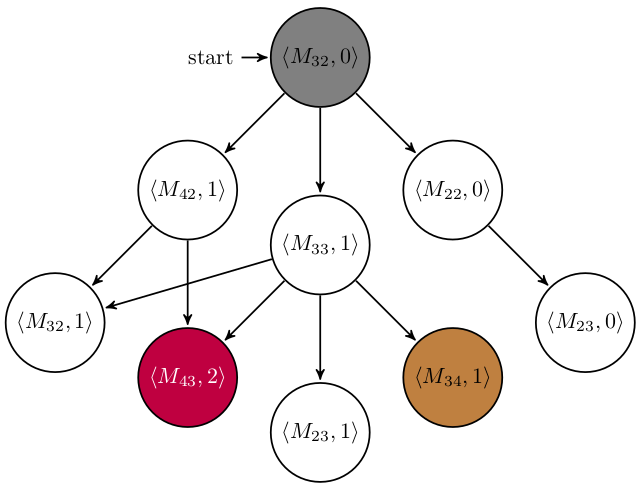
\includegraphics[width=12.0cm]{ej1-graph}
        \caption{El primer elemento de cada nodo revela la ubicación en el mapa y el segundo la cantidad de demoliciones contadas. Dependiendo del orden en que se desencolen los nodos padres, se definirán las ramas azules contra las verdes. El nodo rojo corresponde a un estado cuya rama, de seguir el algoritmo por no llegar ninguna rama al estado final en ese mismo nivel, sería podada. La longitud mínima de valor $2$ nos la da el camino $\langle {M_{33}, M_{34}} \rangle$. Como los puntos de arranque y de salida estarán en el interior del mapa (sino serían paredes), cada rama que pase por el borde tendrá que pasar por \emph{al menos} dos aristas más que la mínima dentro del mapa. Por lo tanto, por razones de espacio omitimos esas ramas en la figura (en el algoritmo sí se consideran). Además de que $P=1$ no permite recorrer el borde más que para salir del interior y luego volver al mismo nodo anterior, lo cual no podría ser mínimo.}
        \label{fig:ej1-graph}
    \end{figure}

    \begin{lstlisting}[caption={Pseudoc\'odigo de la resoluci\'on. En 'candidatos' se guardan los nodos tentativos que quedan por visitar. En dist se guarda la menor distancia que tienen al origen que, por iterar haciendo BFS, es la del primer camino en alcanzar dicho nodo.}]

        dist[m][n][p+1] $\leftarrow$ [m $\times$ n $\times$ (p+1)] * (-1)
        cola<<f, c>, k> candidatos

        dist[origen.f][origen.c][0] $\leftarrow$ 0
        candidatos.encolar(origen, 0)

        $\textbf{Mientras}$ $\neg$candidatos.vacio():
            <ubicacion, k> $\leftarrow$ candidatos.desencolar()
            distancia $\leftarrow$ dist[ubicacion.f][ubicacion.c][k]

            $\textbf{Si}$ ubicacion = destino:
                $\textbf{Devolver}$ distancia

            $\textbf{Para cada}$ vecino <f,c> de ubicacion que este en rango:
                k_vecino $\leftarrow$ k + $\beta$(mapa[vecino.f][vecino.c] es pared)

                $\textbf{Si}$ k_vecino $\leq$ P $\wedge$ dist[vecino.f][vecino.c][k_vecino] = -1:
                    candidatos.encolar(vecino, k_vecino)
                    dist[vecino.f][vecino.c][k_vecino] $\leftarrow$ distancia + 1

        $\textbf{Devolver}$ -1
    \end{lstlisting}


    Veamos que efectivamente el grafo modela bien el problema. En particular nos interesa ver que hay un mapeo directo entre los caminos simples del mapa (formalizados en la introducción a través de \emph{secuencias válidas de vecinos}, que además, como ya dijimos al presentar la representación del grafo, son los que formarán caminos mínimos) y los que no repiten ubicaciones (no solamente simples, sino que para distintos valores de $k$ no pueden repetir una ubicación en común) en el grafo, y que además preserva su secuencia de ubicaciones y longitud final. De esta manera podremos aseverar que encontrar la longitud de un camino mínimo en el grafo es también encontrar la longitud de camino mínimo en el mapa porque existe alguno con esa longitud en él y, si hubiera otro con menor longitud, también lo habría en el grafo con la misma longitud (y por lo tanto el primero no era mínimo). Esto lo podemos formalizar en el siguiente lema:
    \\

    \begin{center}\textbf{\underline{Lema:} }\end{center}
        \textit{Para todo $M_{ij}$ en rango existe en el mapa un camino simple de distancia $n$ desde el punto de inicio $M_{s}$ y que además pasa por $k$ paredes si y sólo si existe un camino de $n$ aristas de distancia entre el vértice $\langle {M_s, 0} \rangle$ y el vértice $\langle {M_{ij},\ k} \rangle$  que recorre vértices asociados a las mismas ubicaciones (todas distintas) en el mismo orden.}
    \\

    Probemos el lema haciendo inducción en el largo $n$ de los caminos. Primero veamos la ida y luego la vuelta:

    \begin{center}$\mathbf{\implies}$\end{center}

    \textbf{\emph{Caso Base (n=1): }} Entonces $M_{ij}$ es vecino en el mapa de $M_s$ en el mapa. Si $M_{ij}$ es pared, entonces $k=1$, de lo contrario $k=0$ porque es el único punto que se visita desde el inicio. Por cómo construimos el grafo, $\langle {M_s, 0} \rangle$ y $\langle {M_{ij},\ k} \rangle$ son siempre adyacentes.
    \\

    \textbf{\emph{Paso inductivo (n$>$1): }} Supongamos un $M_{ij}$ en rango, con al menos un camino de longitud $n$ desde $M_s$ y $k$ demoliciones en él, quiero ver que existe algún camino de longitud $n$ entre $\langle {M_s, 0} \rangle$ y $\langle {M_{ij},\ k} \rangle$ donde la secuencia de primeras componentes de los vértices (todas distintas) coincide con el camino sobre el mapa.
    \\

    \emph{Hipótesis inductiva: } Como $n>1$, no son adyacentes y el camino tiene pasar por algún vecino $M_{xy}$ de $M_{ij}$ antes de terminar en este último. Por HI, a ese subcamino simple entre $M_s$ y $M_{xy}$ de longitud $n-1$ se le corresponde un camino entre $\langle {M_s,\ 0} \rangle$ y $\langle {M_{xy},\ k'} \rangle$ que pasa por las mismas ubicaciones. Como supusimos que el camino entre $M_s$ y $M_{ij}$ en el mapa tiene $k$ demoliciones podemos tomar, usando el mismo subcamino hasta su vecino, $k' = k - \beta(M_{ij}\ es\ pared)$. Esto se puede porque el camino que supusimos es simple, entonces $M_{ij}$ no fue visitado hasta el final y por lo tanto no está en el recorrido de $M_s$ a $M_{xy}$.

    Extendiendo el camino con la arista (existente por ser vecinos y construcción del grafo) entre $\langle M_{xy},\ k' \rangle$ y $\langle M_{ij},\ k''\rangle$ siendo $k'' = k' + \beta(M_{ij}\ es\ pared) = k$, nos queda un camino de longitud $n$ entre $\langle {M_s,\ 0} \rangle$ y $\langle {M_{ij},\ k} \rangle$ que recorre ubicaciones en el mismo orden que el supuesto al principio del paso inductivo. Además, como se corresponde con un camino simple, estas ubicaciones serán todas distintas entre ellas.
    \\

    \begin{center}$\mathbf{\impliedby}$\end{center}

    \textbf{\emph{Caso Base (n=1): }} Similar a la ida, por cómo armamos el grafo sabemos que existe un camino simple de $M_s$ a $M_{ij}$ con longitud 1 en el mapa porque sino $\langle {M_s, 0} \rangle$ y $\langle {M_{ij},\ k} \rangle$ no serían adyacentes en el grafo. Lo mismo para el valor de $k$, que es 0 si $M_{ij}$ no es pared, 1 de lo contrario.
    \\

    \textbf{\emph{Paso inductivo (n$>$1): }} Asumiendo $M_{ij}$ en rango tal que existe un camino que no repite ubicaciones entre vértices de longitud $n$ desde $\langle {M_s, 0} \rangle$ al vértice $\langle {M_{ij},\ k} \rangle$, quiero ver que hay un camino simple de longitud $n$ entre $M_{ij}$ y $M_s$, que pasa por $k$ paredes y las mismas ubicaciones.
    \\

    \emph{Hipótesis inductiva: } También como en la ida, podemos aprovechar que, por construcción y $n>1$, quitando la última arista que hace llegar el camino a $\langle {M_{ij},\ k} \rangle$, podemos formar un subcamino desde $\langle {M_s, 0} \rangle$ hacia algún vecino $\langle {M_{xy},\ k' } \rangle$,  $k'= k-\beta(M_{ij}\ es\ pared)$, de longitud $n-1$.

    Usando HI sobre el subcamino mencionado, sabemos de la existencia de un camino simple de longitud $n-1$ en el mapa que atraviesa $k'$ paredes y va desde $M_s$ hasta $M_{xy}$ recorriendo cada una de las ubicaciones indicadas por nuestro subcamino en el grafo. Y al existir una arista entre $\langle {M_{ij},\ k} \rangle$ y $\langle {M_{xy},\ k' } \rangle$ (tiene que existir por suposición del camino simple del paso inductivo), $M_{ij}$ y $M_{xy}$ son, por construcción del grafo, vecinos en el mapa.

    $M_{ij}$ no pertenece al camino desde $M_s$ hasta $M_{xy}$ que obtuvimos mediante la hipótesis inductiva, porque de hacerlo entonces el camino desde $\langle {M_{s},\ 0} \rangle$ a $\langle {M_{ij},\ k} \rangle$ de donde sale el subcamino sobre el que se aplica la HI tendría ubicaciones repetidas, en particular un vértice $\langle {M_{ij},\ k} \rangle$ y otro de la pinta $\langle {M_{ij},\ k''} \rangle$. Por lo tanto, podemos agregar la arista desde $M_{xy}$ a $M_{ij}$ al camino obtenido y tendríamos un camino simple de longitud $n$ desde $M_{s}$ a $M_{ij}$ con $k'+\beta(M_{ij}\ es\ pared) = k$ demoliciones.
    (al no pertenecer al camino hasta tu su vecino, la última arista se corresponde a un movimiento con demolición).
    \QEDB
    \\

\subsection{Complejidad}

    Previo a las iteraciones, hace falta inicializar la cola de candidatos (implementada con el tipo \href{http://www.cs.northwestern.edu/~riesbeck/programming/c++/stl-summary.html#queue}{\emph{queue}} \footnote{
        http://www.cs.northwestern.edu/\texttildelow riesbeck/programming/c++/stl-summary.html\#queue
    } de la STL de C++) y el arreglo multidimensional con las distancias (implementado con el tipo \href{http://www.cs.northwestern.edu/~riesbeck/programming/c++/stl-summary.html#vector}{\emph{vector}}
    \footnote{
        http://www.cs.northwestern.edu/\texttildelow riesbeck/programming/c++/stl-summary.html\#vector
    }
    , de manera anidada), lo cual cuesta  $\mathcal{O}(1)$ y  $\mathcal{O}(F\times C\times (P+1))$ respectivamente. Las dos inserciones correspondientes al origen se hacen en $\mathcal{O}(1)$.
    \\

    Consideraremos a la variable $n = F\times C\times (P+1)$ como la cantidad de estados posibles.

    Una vez iterando, tenemos una guarda en $\mathcal{O}(1)$ y todas las asignaciones y comparaciones que realizamos en el cuerpo también son $\mathcal{O}(1)$, realizadas $\mathcal{O}(estados) = \mathcal{O}(n)$ veces entendiendo que en peor caso vamos a desencolar todos los estados posibles (como se modifica su distancia al ser encolados, no es posible que vuelvan a evaluarse con distancia -1 y ser reencolados).
    \\

    Se evalúa una guarda que compara ubicaciones en $\mathcal{O}(1)$ al cuerpo de la cual se ingresa una única vez (en caso de haber solución) para retornar la distancia final.
    \\

    Por cada vecino del nodo actual, tendremos que verificar si está en rango y calcular si aumenta la cantidad de demoliciones. Ambas operaciones se hacen en $\mathcal{O}(1)$. Como cada estado tiene 4 vecinos (los correspondientes a moverse en las cuatro direcciones del mapa), esto sucederá $\mathcal{O}(estados) = \mathcal{O}(n) $ veces. Además, hay que actualizar la distancia para los vecinos que no hayan sido actualizados todavía ($\mathcal{O}(1)$ por cada vecino) y agregarlos a la cola de candidatos. La inserción en el tipo $queue$, por ser un \emph{container adaptor}, depende del contenedor sobre el cual se encuentre implementado pero tanto para vectores como para colas doblemente enlazadas es $\mathcal{O}(1)$ amortizado. Asumiendo que todos los vecinos sean siempre vistos por primera vez, nos queda un total de $\mathcal{O}(n)$
    \\

    Sumando todas las complejidades, terminamos con una complejidad final de $\mathcal{O}(n)$ con $n = F\times C\times (P+1)$ y por lo tanto $\mathcal{O}(F\times C\times P)$ que, recapitulando, era nuestra complejidad temporal objetivo.

\newpage
\newpage
\section{Problema 2: Problemas en el camino}

\subsection{Introducción}
	El siguiente obstáculo del grupo de arqueólogos consiste en reconstruir el estado de una balanza de dos platillos con una carga $P$ del lado izquierdo utilizando únicamente pesas de distintas potencias de 3. Además la solución propuesta debe tener complejidad temporal del orden $\mathcal{O}(\sqrt(P))$
	\\

	Por la naturaleza del problema, donde nos interesa determinar únicamente la pertencia de cada potencia en el total de las que usamos para nivelar la balanza (y distinguir a qué lado de la balanza van) la representación del estado final de cada platillo por separado mediante conjuntos disjuntos resulta apropiada. Llamaremos $I$ al conjunto final de las potencias sobre el platillo izquierdo y $D$ a aquellas de la derecha. Además, como cada plato es contrapeso del otro, el estado de la balanza respecto de uno de los platillos se interpreta como su carga menos la del opuesto.
	\\

	A partir de dichas representaciones, dado un valor de $P$, queremos encontrar dos conjuntos disjuntos de potencias de base 3 $I$ y $D$ tales que recreen el estado de la balanza original con una única carga $P$ a la izquierda. Formalmente:

$$
    I,D \subset \{3^n \;|\; n \in \mathbb{N}_0 \} \;\; \land \;\;
    \sum I - \sum D = P \;\; \land \;\;
    I \cap D = \emptyset
$$

	Por ejemplo, para $P$ = 34 el par de conjuntos $\left \langle I,D  \right \rangle$ = $\left \langle \{27,9,1\},\{3\}  \right \rangle$ es solución porque \\
	$\{27,9,1\} \cap \{3\} = \emptyset \ \wedge \ 34 = \sum I - \sum D = (27+9+1)-(3)$.
	\\



\subsection{Solución y Correctitud}
	Para poder determinar $I$ y $D$ es necesario conocer la descomposición polinómica base 3 de $P$. El caso más simple de analizar es cuando $P$ es una potencia de 3 y entonces solamente requerimos de un único elemento para $I$ (es decir, el mismo $P$) y ninguno para $D$. En realidad este es un subcaso de otro más general: que la representación en base 3 de $P$ sea binaria (no haya dígitos que valen 2). Estos casos se pueden resolver fácilmente con $I$ como el conjunto de todos los monomios de la descomposición polinómica, es decir, los dígitos de su representación ternaria. Formalizando, sea $P_{10}$ = $A_3$ = $\left \langle a_{ \left \lfloor{log(P)}\right \rfloor + 1 } \ ... \ a_1, a_0  \right \rangle$ por definición entonces \\

	$P$ = $\sum_{i = 0}^{\left \lfloor{log(P)}\right \rfloor + 1} a_i*3^{i}$ y nos alcanza con tomar $I$ = $\bigl ( \ \bigcup_{i=0}^{\left \lfloor{log(P)}\right \rfloor + 1} \{a_i*3^{i}\} \ \bigr ) \setminus \{0\} \ \ \wedge \ \ D = \emptyset $
	\\

	Sin embargo, hasta ahora obviamos qué sucede si hay coeficientes que valen 2 en la descomposición polinómica de $P$. Retornando a modo ilustrativo al contexto narrativo del problema, no poseemos múltiples pesas de un mismo peso. Es decir que, manteniendo por base la idea para el caso anterior, necesitamos alguna mecánica que garantice la existencia de una solución a costa de cargar valores en $D$ que complementen manipulaciones en $A_3$ para determinar $I$.
	\\

	La algoritmia de la solución trata en recorrer, desde el menos significativo, cada uno de los dígitos $a_i$ de $A_3$, la representación ternaria de $P$, y determinar para ambos conjuntos si $3^{i}$ pertenece a alguno. Como la base está implícita, únicamente guardamos los índices o exponentes $i$ a medida que los recorremos, quedando ordenados crecientemente, y nos encargamos luego de reproducir los verdaderos elementos de $I$ y $D$ elevando 3 a cada exponente. Entonces usamos secuencias $der$ e $izq$ que cumplen:
	\\

	$D = \bigcup_{j=0}^{|der|-1} \{3^{der_{j}}\}  $   \  \ \ \ (idem para $izq$ con $I$)
	\\

	Manteniendo la idea del primer caso, cuando el dígito $a_i$ sea 1 entonces agregamos el exponente $i$ al conjunto $I$, de ser 0 seguimos recorriendo. De este modo seguimos tomando a $A_3$ como base para $I$ aprovechando que tomar los términos de la descomposición polinómica de $P$ para $I$ y $D = \emptyset$ siempre cumple la condición $\sum I$ - $\sum D$ = $P$. Nos queda ver cómo deshacernos de los términos con coeficientes iguales a 2.

	Pero si $a_i$ es 2 lo que hacemos es contar ese exponente para $D$ y provocamos un acarreo hacia el próximo dígito $a_{i+1}$ que pasa a valer $(a_{i+1} + 1) \ mod \ 3$. Se puede ver que puede llegar a caer en otro dígito que ya valía 2, generando más acarreos hasta caer en un dígito que valga 1 (teniendo que generar otro acarreo por la idea del algoritmo) ó 0, 'tomando' el acarreo y sumando para $I$ la diferencia que creamos al agregar el exponente original $i$ en $D$, y poder seguir aplicando el mismo método en los próximos dígitos.

	Esto, visto desde la resta de ambos conjuntos, significa sumar $3^{i}$ tanto para $\sum I$ como $\sum D$. Por invariante de la iteración (hasta ahora solamente nos ocupamos de los dígitos anteriores, por lo que $i \notin der \cup izq$), si consideramos las sumas de ambos conjuntos como una descomposición polinómica base 3, este término valía 0 para $\sum D$ y $2*3^{i}$ para $\sum I$, quedando $3^{i}$ y $(2+1)*3^{i} = 3^{i+1}$ respectivamente y viendo además que de este modo no repetimos exponentes entre $I$ y $D$ ($3^i$ pertenece a $D$ pero no a $I$).
	\\
	
	Por lo tanto, distribuyendo restas algebráicamente válidas de la pinta ($3^{i}-3^{i}$) entre $I$ y $D$ pudimos mantener la idea que satisfacía originalmente $\sum I$ - $\sum D$ = $P$ partiendo de $D$ = $\emptyset$ e $I$ como los monomios de la descomposición polinómica base 3 de $P$, de tal modo que fuimos 'pateando' los términos con coeficientes de valor 2 a términos de mayor grado y manteniendo los dos conjuntos con intersección vacía. En el pseudocódigo siguiente se ve más claro incluso por qué nunca se cuenta el mismo exponente para ambos conjuntos.
\\
\\
\lstset{basicstyle=\large}
\begin{lstlisting}
    hayCarry $\leftarrow$ false				
    exponente $\leftarrow$ 0

    for digito in <$a_0$... $a_{ \left \lfloor{log(P)}\right \rfloor + 1}$>:
        if hayCarry:
            digito $\leftarrow$ digito + 1
            digito $\leftarrow$ digito $mod$ 3
            hayCarry $\leftarrow$ true if digito es 0

        if digito es 2:
            agregar exponente al final de der
            digito $\leftarrow$ 0
            hayCarry

        else if digito es 1:
            agregar exponente al final de izq

        exponente $\leftarrow$ exponente + 1

    if hayCarry:
         agregar exponente al final de izq

\end{lstlisting}

	%Proposición:
	%\\
	%Q($j$): Para todo dígito $a_j$ iterado, con $0 \leq j < \left \lfloor{log(P)}\right \rfloor + 1$, tras su iteración las secuencias $der$ e $izq$ son disjuntas y se cumple que:
	%\\
	%
	%$\sum_{i=0}^{|der|-1} 3^{der_i} + \beta(hayCarry)*3^{j+1} - \sum_{i=0}^{|izq|-1} 3^{izq_i} = \sum_{i=0}^{j} a_i*3^{i} $
	%\\
	%
	%Probémoslo por inducción en $j$. Sea el caso base:
	%
	%Q($0$): En la primer iteración se comienza sin $carry$ siempre.
	%
	%\begin{itemize}
	%\item Si $a_0$ = 0 entonces $der$ = $izq$ = $[]$ y no se genera $carry$. Por lo tanto vale la igualdad porque ambos lados son nulos y ambas secuencias siguen vacías y por lo tanto disjuntas.
	%\item Si $a_0$ = 1 entonces $izq$ = $[0]$, $der$ = $[]$ y tampoco se genera $carry$. $der$ e $izq$ siendo disjuntas y vale que $3^{0} + \beta(false)*3^{1} - 0 = 1 = 1*3^{0}$-
	%\item Si $a_0$ = 2 entonces $der$ = $[0]$, $izq$ = $[]$ y se genera $carry$. Al igual que en el caso anterior, siguen siendo disjuntos. También vale la igualdad porque $0 + \beta(true)*3^{1} - 3^{0} = 3 - 1 = 2*3^{0} = 2$
	%\end{itemize}
	%
	%Por lo tanto, en todos los casos sabemos que se preservan ambas condiciones.
	%\\
	%
	%Paso inductivo:
	%Asumo válido Q($n-1$), quiero ver que vale Q($n$).
	%En la iteración anterior puede haberse, o no, producido $carry$. Separamos en casos, empezando con el caso en que no hay:
	%
	%\begin{itemize}
	%\item Si $a_n$ = 0 entonces no se modifica ninguna de las secuencias ni se genera $carry$, por HI entonces estas condiciones cumplen la igualdad y la disjunción.
	%\item Si $a_n$ = 1 entonces $der = pre(der)++[n] $, $izq = pre(izq)$ y no se genera $carry$. Por HI sabemos que vale:   \\
	%$\sum_{i=0}^{|der|-2} 3^{der_i} - \sum_{i=0}^{|izq|-1} 3^{izq_i} = \sum_{i=0}^{n-1} a_i*3^{i} $
	%\\
	%Usando que $3^{|der|-1} = 3^{n} = a_{n}*3^{n}$, sumando de ambos lados:
	%\\
	%$\sum_{i=0}^{|der|-2} 3^{der_i} + 3^{|der|-1} - \sum_{i=0}^{|izq|-1} 3^{izq_i} = \sum_{i=0}^{n} a_i*3^{i} + 3^{n} $
	%\\
	%$\sum_{i=0}^{|der|-1} 3^{der_i} - \sum_{i=0}^{|izq|-1} 3^{izq_i} = \sum_{i=0}^{n+1} a_i*3^{i}$
	%Que es
	%\item Si $a_j$ = 2 entonces
	%\end{itemize}

\newpage
\subsection{Complejidad}
	El pseudocódigo no incluye el ciclo final que se encarga de convertir $der$ e $izq$ en la secuencia ordenada de elementos de $I$ y $D$. Esto se hace iterando de principio a fín cada vector y devolviendo por salida estándar $3^{\ elem \ actual}$ en cada iteración. Considerando a la operación pow($base$, $exp$) constante, el costo del ciclo es $\mathcal{O} (|der| + |izq|)$. Más adelante vamos a ver que ambas longitudes son orden de $log_3(P)$.
	
	Otra cosa que no incluímos en el pseudocódigo (por una leve simplificación) es cómo se consigue la representación base 3 de $P$ que iteramos. La guarda original del ciclo corresponde a:
	
	%\lstset{basicstyle=\large}
	\begin{lstlisting}
	[...]
	while P > 0:
        	digito $\leftarrow$ P mod 3
        	P $\leftarrow$ P / 3
	[...]
	\end{lstlisting}
	
	Por lo tanto en cada iteración conseguimos, mediante el algoritmo clásico de conversión de base mediante división, el próximo dígito. Cuando $P \leq 0$ entonces el ciclo termina y como $P$ decrementa a un tercio en cada iteración, esto significa que el ciclo se ejecuta un orden de $log_3(P)$ veces. 
	\\
	
	En el cuerpo del ciclo todas las operaciones aritméticas que se realizan son constantes en complejidad temporal (asumimos $mod$ incluída), pero también se realiza hasta una inserción en las secuencias $izq$ y $der$ por ciclo. Ambas secuencias las implementamos con el tipo $vector$ y, por lo tanto, la inserción corresponde a la operación $push\_back(elem)$. Esta operación tiene complejidad temporal constante amortizada, aunque podrían suceder 'reubicaciónes' que hicieran que para esa llamada en particular el costo sea lineal. Vamos a analizar partiendo de la complejidad amortizada, considerando que también se podría usar un array de tamaño $\left \lfloor{log_3(P)}\right \rfloor + 2$ ($\left \lfloor{log_3(P)}\right \rfloor + 1$ por la representación de P en base 3 y un 'bit' más por si hay un acarreo) y tener acceso constante en general.
	
	Entonces nuestro ciclo se va a ejecutar $\mathcal{O} (log(P))$ veces, con guarda y cuerpo $\mathcal{O} (1)$. Lo que nos deja un ciclo con complejidad temporal $\mathcal{O} (log(P))$ y luego un proceso encargado de imprimir salidas estándar de costo $\mathcal{O} (|der| + |izq|)$. Pero, como ya anticipamos, ambas longitudes son $\mathcal{O} (log(P))$ porque solamente vamos a iterar una cantidad logarítmica (respecto de P) de dígitos y no puede haber ninguno (por correctitud respecto del enunciado) repetido en ambos vectores. Por lo tanto nos queda una complejidad final de $\mathcal{O} (log(P))$.
	\\
	
	Nos resta ver que $\mathcal{O} (log(P))$ = $\mathcal{O} (\sqrt(P))$ para probar que cumplimos con los requisitos de complejidad del problema inicial.
	
	Por propiedades de logarítmos $log(P) = 2log(\sqrt(P))$ y usando que $\forall \ x > 0, \ log(x) < x$ nos queda que $ P > 0 \Longrightarrow log(P) < 2\sqrt(P)$, y por lo tanto podemos asegurar $log(P) \in \mathcal{O} (\sqrt(P))$. 

\subsection{Análisis experimental}

	Al ser $P$ la única variable sobre la cual depende del funcionamiento general del algoritmo, sobre la cual se sugiere por enunciado interpretar un rango $1 \leq P \leq 10^{15}$, nuestros tests para analizar dicho funcionamiento se centran en probar distintos valores de esta variable. Además, como cada rama dentro del cuerpo del $for$ del algoritmo tiene el mismo orden de complejidad (considerando las inserciones en los vectores en su complejidad amortizada, como ya explicamos anteriormente), no se distinguen 'peores casos' para valores de $P$.
	\\

\begin{figure}[H]
    \centering
    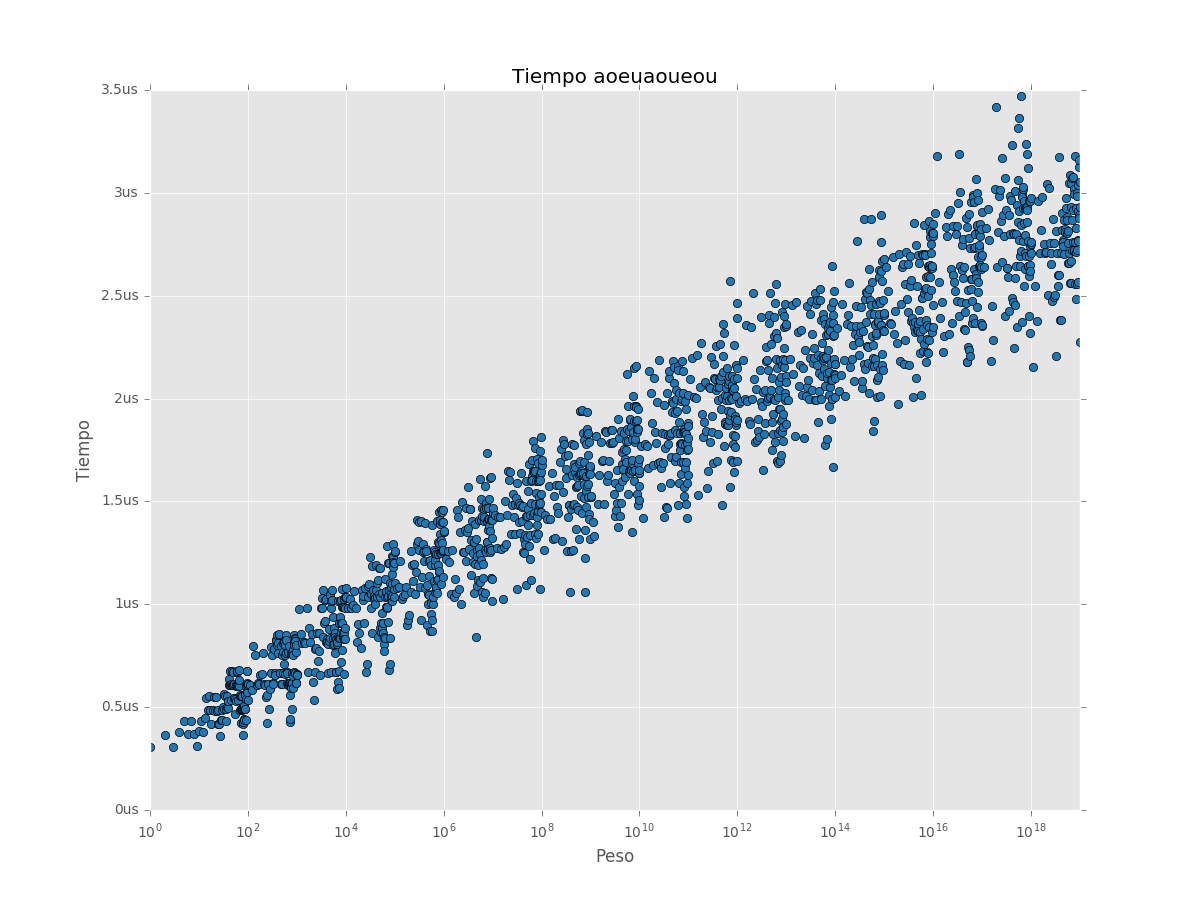
\includegraphics[width=\textwidth]{ej2}
    \caption{Tiempo de ejecución del algoritmo en función de P}
    \label{fig:ej2-fig}
\end{figure}

Los casos se generan con el criterio de distribuir, en los intervalos $[10^i$..$10^i+1]$ para $0 < i < 19$ (la cota superior se debe a la capacidad del tipo \emph{uint64_t} de $c++$), un caso cada $10^{i-1}$ valores de $P$ \footnote{Para el intervalo de 0 a 10, son 10 mediciones para cada valor entero.}. La razón de esto es que en la sección anterior sugerimos una complejidad de orden logarítmico sobre el tamaño de la variable $P$ y una manera de contrastar empíricamente esto es notar un crecimiento lineal en el tiempo de ejecución para un eje de coordenadas exponencial para $P$, como podemos apreciar efectivamente en la figura \ref{fig:ej2-fig}.


\newpage
\section{Problema 3: Escapando}

Luego de juntar todas las piezas, Indy llega a la cruz marcada en el mapa y se encuentra con una red de carritos que parecen dirigirse hacia afuera de la fortaleza, cuando de repente la fortaleza se empieza a derrumbar, asi que no tiene mas opcion que usar los carritos para escapar.

Los parametros de entrada son los siguientes

	\begin{itemize}
		\item Dos numeros N y M que representan la cantidad de estacion y la cantidad de vias.
		\item M lineas, las cuales contienen 3 enteros A,B y C que representan que ir de A a B tarda C segundos. Las estaciones se encuentran numeradas desde 1 hasta N
    \end{itemize}

Los parametros de salida son los siguientes

	\begin{itemize}
	\item Un entero T que indica el tiempo minimo necesario para escapar. En caso de que no haya camino, este valor debera ser -1
	\item Asumiendo que haya solucion, la siguiente linea contendra la cantidad de estaciones a recorrer.
	\item Asumiendo que haya solucion. esta linea debera contener la secuencia de las estaciones a recorrer.

	\end{itemize}	

La solucion tiene que tener una complejidad temporal de $\mathcal{O}(N^{2})$ o mejor.

\subsection{Solución}

Vamos a modelar el problema mediante grafos dirigidos. Si pensamos a las estaciones como los vertices y el tiempo necesario para ir de una estacion a otra como el peso de la arista dirigida correspodiente, resulta que el problema se reduce a calcular el camino minimo entre la estacion 1 (donde estan ubicados) y la estacion n , a la cual quieren llegar.

%Si bien parece trivial, no sabemos si hace falta aclararlo.
La longintud del camino es la sumatoria de las aristas que usa, por lo dicho anteriormente esto equivale al tiempo necesario para recorrerr dicho camino, esto seria la primera linea de la salida

Para resolver el problema vamos a aplicar un algoritmo de camino minimo en grafos, en este caso vamos a usar Djistra

   \begin{lstlisting}
   visitados <-vector[n,false]
   tiempoMin <-vector[n, $\infty$]

   while

   \end{lstlisting}



\newpage
\section{Códigos Fuente}
\subsection{Ejercicio 1}

\lstset{language=C++,
                basicstyle=\ttfamily,
                keywordstyle=\color{blue}\ttfamily,
                stringstyle=\color{red}\ttfamily,
                commentstyle=\color{green}\ttfamily,
                morecomment=[l][\color{magenta}]{\#}
}

\begin{lstlisting}[ basicstyle=\small]
    #include <math.h>
    #include <stdint.h>
    #include <algorithm>
    #include <cassert>
    #include <iostream>
    #include <map>
    #include <queue>
    #include <set>
    #include <tuple>
    #include <vector>

    using namespace std;

    // Hay 2^(N+M) estados posibles
    typedef struct estado_t {
        // Para todo, true = del lado derecho
        vector<bool> arq;
        vector<bool> can;
        bool linterna = false;

        estado_t(){};
        estado_t(uint32_t n, uint32_t m) : arq(n), can(m) {}

        // La priority_queue requiere <
        bool operator<(const struct estado_t &o) const {
            return tie(linterna, arq, can) < tie(o.linterna, o.arq, o.can);
        }
        bool operator==(const struct estado_t &o) const {
            return tie(linterna, arq, can) == tie(o.linterna, o.arq, o.can);
        }
    } estado;

    vector<uint32_t> arq;
    vector<uint32_t> can;

    bool agregarCandidato(map<estado, uint32_t> &dist,
                          set<pair<uint32_t, estado>> &candidatos, estado &hijo,
                          uint32_t peso);

    int64_t tiempoMinimo(const vector<uint32_t> &arq, const vector<uint32_t> &can) {
        // Empiezan todos del lado izquierdo
        estado inicial(arq.size(), can.size());
        estado objetivo;
        objetivo.arq = vector<bool>(arq.size(), true);
        objetivo.can = vector<bool>(can.size(), true);
        objetivo.linterna = true;

        // Distancia minima hasta el estado
        map<estado, uint32_t> dist;
        dist.insert({inicial, 0});

        // Mantenemos la lista de candidatos a explorar,
        // y vemos siempre el mas cercano primero
        set<pair<uint32_t, estado>> candidatos;
        candidatos.insert(make_pair(0, inicial));

        int64_t res = -1;
        while (!candidatos.empty()) {
            auto p = candidatos.begin();
            uint32_t costo = p->first;
            estado nodo = p->second;
            candidatos.erase(p);

            // Llegamos a la solucion
            if (nodo == objetivo) {
                res = costo;
                break;
            }

            // Hacemos un population count
            uint32_t arqIzq = 0;
            uint32_t canIzq = 0;

            for (uint32_t i = 0; i < arq.size(); i++)
                if (nodo.arq[i])
                    arqIzq++;
            for (uint32_t i = 0; i < can.size(); i++)
                if (nodo.can[i])
                    canIzq++;

            // Checkeamos que no sea un caso invalido
            if ((arq.size() - arqIzq > 0) &&
                (arq.size() - arqIzq) < (can.size() - canIzq)) {
                continue;
            }
            if (arqIzq > 0 && arqIzq < canIzq) {
                continue;
            }

            // Generamos los pasos posibles a partir de donde estamos
            estado hijo = nodo;
            hijo.linterna = !hijo.linterna;

            for (uint32_t i = 0; i < arq.size(); i++) {
                // Checkear si esta de este lado
                if (nodo.arq[i] != nodo.linterna)
                    continue;

                hijo.arq[i] = !nodo.linterna;
                for (uint32_t j = i; j < arq.size(); j++) {
                    if (nodo.arq[j] != nodo.linterna)
                        continue;
                    hijo.arq[j] = !nodo.linterna;

                    // El movimiento siempre cuesta la menor de las velocidades
                    uint32_t costoExtra = max(arq[i], arq[j]);
                    uint32_t distancia = costo + costoExtra;

                    // Agregamos este hijo a la lista
                    agregarCandidato(dist, candidatos, hijo, distancia);

                    if (i != j)
                        hijo.arq[j] = nodo.linterna;
                }
                // Lo volvemos a como estaba
                hijo.arq[i] = nodo.linterna;
            }

            for (uint32_t i = 0; i < can.size(); i++) {
                // Checkear si esta de este lado
                if (nodo.can[i] != nodo.linterna)
                    continue;

                hijo.can[i] = !nodo.linterna;
                for (uint32_t j = i; j < can.size(); j++) {
                    if (nodo.can[j] != nodo.linterna)
                        continue;
                    hijo.can[j] = !nodo.linterna;

                    // El movimiento siempre cuesta la menor de las velocidades
                    uint32_t costoExtra = max(can[i], can[j]);
                    uint32_t distancia = costo + costoExtra;

                    // Agregamos este hijo a la lista
                    agregarCandidato(dist, candidatos, hijo, distancia);

                    if (i != j)
                        hijo.can[j] = nodo.linterna;
                }
                // Lo volvemos a como estaba
                hijo.can[i] = nodo.linterna;
            }

            for (uint32_t i = 0; i < arq.size(); i++) {
                // Checkear si esta de este lado
                if (nodo.arq[i] != nodo.linterna)
                    continue;

                hijo.arq[i] = !nodo.linterna;
                for (uint32_t j = 0; j < can.size(); j++) {
                    if (nodo.can[j] != nodo.linterna)
                        continue;
                    hijo.can[j] = !nodo.linterna;

                    // El movimiento siempre cuesta la menor de las velocidades
                    uint32_t costoExtra = max(arq[i], can[j]);
                    uint32_t distancia = costo + costoExtra;

                    // Agregamos este hijo a la lista
                    agregarCandidato(dist, candidatos, hijo, distancia);

                    hijo.can[j] = nodo.linterna;
                }
                // Lo volvemos a como estaba
                hijo.arq[i] = nodo.linterna;
            }
        }

        return res;
    }
\end{lstlisting}
\begin{lstlisting}[ basicstyle=\small]
    bool agregarCandidato(map<estado, uint32_t> &dist,
                          set<pair<uint32_t, estado>> &candidatos, estado &hijo,
                          uint32_t distancia) {
        auto s = dist.find(hijo);
        if (s != dist.end()) {
            // El hijo ya tiene una distancia
            // lo agregamos solo si la distancia resultante es menor
            uint32_t distVieja = s->second;

            if (distancia < distVieja) {
                // Hay que borrar la posicion en la cola de candidatos
                // para insertarlo de nuevo
                auto p = candidatos.find({distVieja, hijo});
                candidatos.erase(p);
                dist.erase(dist.find(hijo));
            } else {
                // La distancia anterior ya era mejor que venir por este camino
                return false;
            }
        }

        dist.insert({hijo, distancia});
        candidatos.insert({distancia, hijo});

        return true;
    }
\end{lstlisting}

\newpage
%-------------------------------------------------------------------
%-------------------------------------------------------------------
%-------------------------------------------------------------------
\subsection{Ejercicio 2}

\begin{lstlisting}[ basicstyle=\small]
      #include <math.h>
      #include <stdint.h>
      #include <iostream>
      #include <set>
      #include <vector>

      using namespace std;

      uint64_t peso;

      void balancear(uint64_t peso, vector<uint8_t> &izq, vector<uint8_t> &der) {
          // peso = sum(3^izq) - sum(3^der)

          bool carry = false;
          uint8_t exponente = 0;

          // Recorremos los dígitos en base 3, empezando por el menos significativo
          while (peso > 0) {
              uint8_t digito = peso % 3;
              peso /= 3;

              // Le sumamos una pesa al dígito anterior, y quedo un carry
              if (carry) {
                  digito += 1;
                  digito %= 3;

                  // Checkear si se genero otro carry mas
                  carry = digito == 0;
              }

              if (digito == 2) {
                  // A cada dígito '2' del peso hay que sumarle 1

                  // Agregamos una pesa con este exponente
                  der.push_back(exponente);

                  // Actualizamos el peso
                  digito = 0;
                  carry = true;

              } else if (digito == 1) {
                  // Si quedo un 1 agregamos una pesa del otro lado, para
                  // contrarestarlo
                  izq.push_back(exponente);
              }

              exponente++;
          }

          if (carry)
              izq.push_back(exponente);
      }
\end{lstlisting}

\newpage
%-------------------------------------------------------------------
%-------------------------------------------------------------------
%-------------------------------------------------------------------
\subsection{Ejercicio 3}

\begin{lstlisting}[ basicstyle=\small]
#include <stdint.h>
#include <algorithm>
#include <iostream>
#include <map>
#include <set>
#include <vector>
#include <math.h>

using namespace std;

typedef struct mkp_object_t {
    uint64_t id;
    uint64_t weight;
    int64_t value;
} mkp_object;

vector<uint64_t> bins(3,0);
vector<mkp_object> objects;

uint64_t mkp(vector<uint64_t> bins, vector<mkp_object> const &objetos,
             vector<vector<uint64_t>> &resultIds) {
    // O(pi(bins) * count(objects) )

    // Si hay menos de 3 mochilas, consideramos las siguientes como
    // de tamano 0

    // Para cada combinacion de k_i pesos de las mochilas, con 0 <= k_i <=
    // capacidad(i)
    // calculamos el mayor valor conseguible ocupando exactamente ese espacio
    //
    // En cada combinacion, para cada 0 <= j <= cantidad de objetos,
    // calculamos el optimo usando los primeros j objetos.

    vector<vector<vector<vector<int64_t>>>> mejorValor(
        bins[0] + 1,
        vector<vector<vector<int64_t>>>(
            bins[1] + 1,
            vector<vector<int64_t>>(bins[2] + 1,
                                    vector<int64_t>(objetos.size() + 1, -1))));

    vector<vector<vector<vector<int64_t>>>> binObjeto(
        bins[0] + 1,
        vector<vector<vector<int64_t>>>(
            bins[1] + 1,
            vector<vector<int64_t>>(bins[2] + 1,
                                    vector<int64_t>(objetos.size() + 1, -1))));

    // 0 objetos en mochilas de tamano 0 tienen valor 0
    mejorValor[0][0][0][0] = 0;

    int64_t valorMax = 0;
    vector<uint64_t> sizesMax(3, 0);

    for (uint64_t w0 = 0; w0 <= bins[0]; w0++) {
        for (uint64_t w1 = 0; w1 <= bins[1]; w1++) {
            for (uint64_t w2 = 0; w2 <= bins[2]; w2++) {
                // Para cada primeros j objetos buscamos el máximo
                for (uint64_t j = 1; j <= objetos.size(); j++) {
                    const mkp_object &obj = objetos[j - 1];

                    // Decidimos si conviene poner el objeto en una mochila o no
                    // usarlo
                    int64_t valCandidato, valor = mejorValor[w0][w1][w2][j - 1];

                    valCandidato = obj.weight > w0 ? -1 :
                        mejorValor[w0 - obj.weight][w1][w2][j - 1] + obj.value;
                    if (valor < valCandidato) {
                        binObjeto[w0][w1][w2][j] = 0;
                        valor = valCandidato;
                    }

                    valCandidato = obj.weight > w1 ? -1 :
                        mejorValor[w0][w1 - obj.weight][w2][j - 1] + obj.value;
                    if (valor < valCandidato) {
                        binObjeto[w0][w1][w2][j] = 1;
                        valor = valCandidato;
                    }

                    valCandidato = obj.weight > w2 ? -1 :
                        mejorValor[w0][w1][w2 - obj.weight][j - 1] + obj.value;
                    if (valor < valCandidato) {
                        binObjeto[w0][w1][w2][j] = 2;
                        valor = valCandidato;
                    }

                    mejorValor[w0][w1][w2][j] = valor;
                }

                // Mantenemos el máximo valor visto
                if (valorMax < mejorValor[w0][w1][w2][objetos.size()]) {
                    valorMax = mejorValor[w0][w1][w2][objetos.size()];
                    sizesMax = {w0, w1, w2};
                }
            }
        }
    }

    // Escribimos los ids del resultado
    resultIds.resize(bins.size());

    for(uint64_t j=objetos.size(); j > 0; j--) {
        int64_t bin = binObjeto[sizesMax[0]][sizesMax[1]][sizesMax[2]][j];
        if (bin != -1) {
            resultIds[bin].push_back(objetos[j-1].id);
            sizesMax[bin] -= objetos[j-1].weight;
        }
    }

    // Como recorrimos los objetos desde el ultimo hay que invertir el array
    // (se pide ordenado)
    for (auto &v : resultIds) {
        reverse(v.begin(), v.end());
    }
    return valorMax;
}
\end{lstlisting}


\appendix

%\newpage
%\bibliography{bibliography}{}
%\bibliographystyle{plain}

\end{document}
